This example is presented to introduce \textit{bioptim}'s ability to provide real-time estimation of biomechanical variables.
The goal was to perform a real-time estimation of dynamically consistent joint kinematics and muscle forces, using a moving horizon estimation (MHE). 
A shoulder elevation motion was performed with a 4-DoFs ($q$) arm actuated by 19 Hill-type muscle elements.
The control inputs of the model were the muscle activations ($a$).
The MHE implementation consists in splitting the OCP into a succession of smaller one for processing fixed-size subsets of the tracking data moving forward in time. 
Each time one subproblem is solved, a new measurement is added, the oldest one is discarded and a new subproblem is defined. 
Due to their similarities, the solution of the previous OCP is a good initial guess to the new one. 
The dynamical consistency of the final solution is enforced by continuity constraints on the initial state. 
Each objective function (Eq.~\ref{eq:ocp_exMHE}) was written as the sum of three terms: tracking reference joint angles ($q^*$), states and muscle activations regularizations (i.e., least-square criteria): 

\[ 
\resizebox{0.9\columnwidth}{!}{$ 
\begin{aligned}
\mathcal{J} = &\int_t^{t+t_{mhe}}\underbrace{\omega_1´(\|q - q^*\|^{2})}_{\mathtt{TRACK\_STATE}}~ 
+ ~ \underbrace{\omega_2\|q\|^2}_{\mathtt{MIN\_STATE}} 
+ ~ \underbrace{\omega_3\|a\|^2}_{\mathtt{MIN\_ACTIVATION}}~dt, 
\end{aligned}  
$}  
\addtag  
\label{eq:ocp_exMHE}  
\]  

\noindent where $\omega_1 =10^5$, $\omega_2 = 10^2$, $\omega_3 = 10^4$ and $t_{mhe}$ is duration of each sub-problem. 

In this example, reference data of an $8~s$ series of four arm elevations were generated at 100~Hz, by computer simulation.
Centered Gaussian noise (mean = 0, std = $0.005q^*(t)$) was added to $q^*$, to simulate experimental-like joints angle measurements.
Using a windows size of 7 nodes, the estimator ran at about 33~Hz (one in three reference data frame was sent to the estimator to simulate experimental-like conditions), i.e., two and half times faster than standard biofeedback (13~Hz, \cite{kannape2013biofeedback}).
The MHE was able to forecast the movement kinematics with a root mean square error of $1.33\pm0.52\text{~}^{\circ}$ (Fig.~\ref{fig:joint_angles_MHE}) and to provide a realistic estimation of muscle forces close to the ground truth with a root mean square error of $10.6\pm13.6\text{~}N$ (Fig.~\ref{fig:muscle_forces_MHE}, only the muscles with significative action (peaks force $>$ 15~N) are represented).  
 
\begin{figure*}[t!] 
\centering 
\includegraphics[width=\textwidth]{figures/joint_angles_MHE.pdf}\\ 
\caption{Time series of estimated joint angles (blue) and noisy reference joint angles (orange).} 
\label{fig:joint_angles_MHE} 
\end{figure*} 

\begin{figure*}[t!] 
\centering 
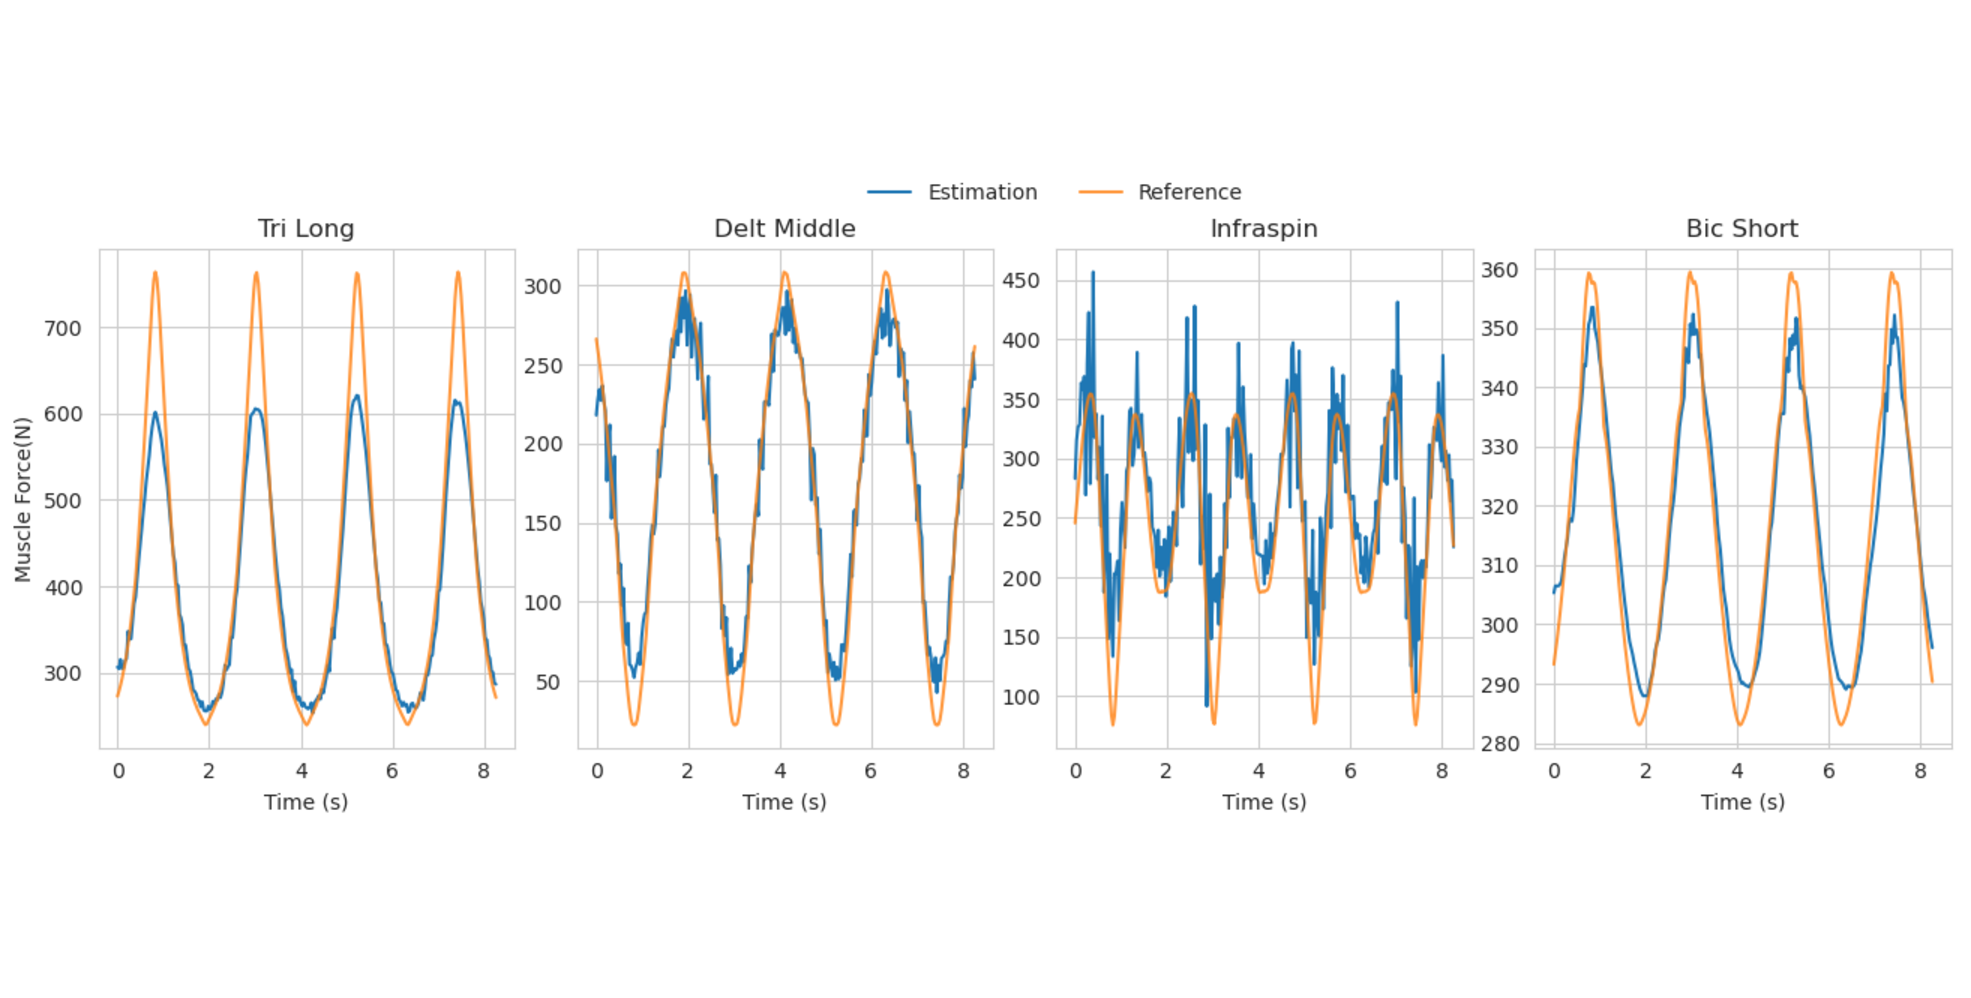
\includegraphics[width=\textwidth]{figures/Muscle_Forces_MHE.pdf}\\ 
\caption{Time series of estimated muscle forces (blue) and ground truth muscle forces (orange). 
Only the muscles with significative action (peaks force $>$ 15~N) are represented.
Muscle abbreviations stand for (from left to right and top to bottom): Triceps Long head, Lateral and Medial, Brachial, Brachioradialis, Deltoid Anterior and Middle, Infraspinatus, Subscapularis, Biceps Brachial Long and Short head.} 
\label{fig:muscle_forces_MHE} 
\end{figure*} 

